\include{dog16template}

\newcommand{\x}{\mathbf{x}}
\newcommand{\y}{\mathbf{y}}
\newcommand{\z}{\mathbf{z}}
\newcommand{\blambda}{\boldsymbol{\lambda}}
\newcommand{\bmu}{\boldsymbol{\nu}}
\usepackage{color}
\usepackage{tikz}
\usepackage{pgfplots}
\usetikzlibrary{positioning}
\usetikzlibrary{arrows}
\usepackage[margin=1in]{geometry}
\usepackage{multirow,booktabs}


\begin{document}
\lecture{3}{January 4, 2017}{Mohamad El laz}

%Notes
\section{Introduction}
The goal of this lecture is to study a different distributed problem from what we have studied until now.In the previous lectures we saw how users where able to choose their own routes and how their choices affected the behavior of the system.

In this lecture, we study the case where routes are fixed and users can only decide what to route.For that the title of our lecture is "Bandwidth sharing over the Internet".

\section{Problem definition}
Let us consider the case where a user wants to download some contents from the Internet (Figure~\ref{fig:1}).

% Graph
\begin{figure}[!h]
	\centering
	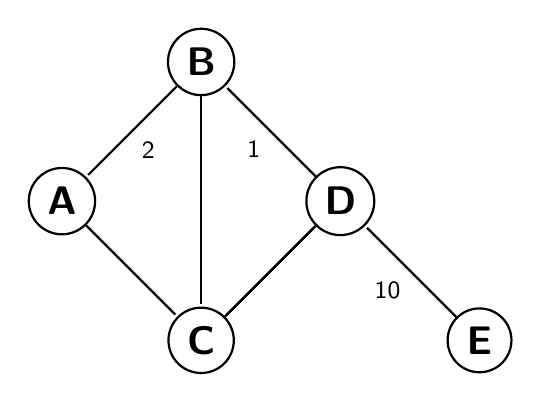
\begin{tikzpicture}[shorten >=1pt, auto, thick,
	auto,node distance=2.5cm,
	thick,main node/.style={circle,draw,font=\sffamily\Large\bfseries}]
	\node[main node] (1) {B};
	\node[main node] (2) [below left of=1] {A};
	\node[main node] (3) [below right of=2] {C};
	\node[main node] (4) [below right of=1] {D};
	\node[main node] (5) [below right of=4] {E};
	\path[every node/.style={font=\sffamily\small}]
	(1) edge node  {2} (2)
	edge node {} (3)
	(2) edge node {} (3)
    (3) edge node  {} (4)
	(4) edge node  {} (3)
	edge node {1} (1)
	(5)edge node {10} (4)	;
	\end{tikzpicture}
	\caption{server-client connection} \label{fig:1}
\end{figure}

In order to download some contents from the Internet, a connection might be established between the user and the server, this process is controlled by TCP (\textit{Transmission Connection Protocol}).TCP is a connection-oriented protocol, it determines how to break application data into packets that networks can deliver, sends packets to and accepts packets from the network layer, manages flow control, and handles retransmission of dropped or garbled packets as well as acknowledgment of all packets that arrive.

In this example the route is fixed by the Internet provider and there is no fixed amount of traffic (the more, the better). We consider a first client (c1) downloading a file from the server on route A-B-D-E, a first constraint is that the download speed won't exceed 1 Mb/s. The second constraint would be that another client (c2) is trying to download from the same source (Route A-C-D-E) or he is sharing the same link (Route C-B-D-E).To see how the Internet splits the downloading rate we will consider a general model.

\section{A general model for the problem}

To be fair with all users, we should maximize their global happiness expressed by the rate at which their files are downloaded.A very common way to model users happiness is by an increasing concave function (Figure~\ref{fig:2}):
\begin{itemize}
	\item Increasing as the more value users have the happier they are.
	\item Concave because the rate given to users obeys the law of diminishing return.
\end{itemize}

%law of diminishing return
\begin{remark}
	The law of diminishing return is a commonly used concept in the field of economy. Let us consider the diminishing marginal utility (happiness) of income, which means that as income increases, individuals gain correspondingly a smaller increase in happiness. To explain it better let's see this example below.
	
	If you have zero income and gain 10€ per day, this will improve your living standards significantly as you will be able to pay for basic necessity of life (i.e. food). 
	
	However, if you already gain 500€ a day, an extra 10€ has a proportionately smaller increase in utility (it doesn’t significantly affect your standard of living and happiness).
	
	Now, if you are earning 15,000€ a day, you would hardly notice an extra 10€. Therefore, we say that the marginal utility of an extra 10€ at this income level is very limited.
	
	The same idea is applied on the marginal happiness of users downloading from Internet, where the user is unhappy when there is no downloading rate but bit happier if the rate is higher. Of course when having a high connection, the user will be happy with a higher connection (double rate) but not happy as twice.
	
	Thus, as income increases, the extra marginal benefit to individuals declines.

\end{remark}

%Concave function
\begin{figure}[h]
	\centering
	\begin{tikzpicture}
	\begin{axis}[domain=-4:4, samples=1000,
	restrict y to domain=0:4,legend pos=north west]
	\addplot [color=blue]    {(ln(x)};
	\end{axis}
	\end{tikzpicture}
	\caption{An increasing concave function} \label{fig:2}
\end{figure}
\subsection{Solving the problem by the Lagrange multipliers method}
We will just identify the users as the routes as if users can't decide the routes (one user corresponds to one route):
\begin{itemize}
	\item $R$ is the set of all routes/users.
	\item $E$ is the set of edges.
	\item $l \in r$ where link $l$ is a part of route $r$.
	\item $C_l$ is the capacity of link $l$ (the maximum rate that $l$ can achieve).
	\item $U_r(x_r)$ is the utility of user $r$ for downloading at rate $x_r$.
\end{itemize}
Thus our objective is to maximize the sum of users happiness.

The optimization problem can be modeled as follows:
\begin{equation}
\begin{aligned}
& {\text{maximize}}
& &  \sum_{r \in R} U_{r}(x_{r}) \\
& \text{subject to}
& & \sum\limits_{r|l \in r} x_{r} \leq C_{l},\ \forall l \in E\\
&      &&  x_{r} \geq 0,\ \forall r \in R\\
\end{aligned}
\label{Max}
\end{equation}
Where $y_l=\sum\limits_{r | l \in r} x_r$.

For convenience, we also assume that $U_r(x_r)$ is strictly concave, continuously differentiable on $(0,\infty)$, and satisfies $U'_r(0) = \infty$ and $U'_r(\infty) = 0$.

This is a problem for which we know that the Lagrangian is a necessary and sufficient condition (as if the sum of concave functions is a concave function and the constraints are linear), so we can apply \textit{Theorem 2} of lecture 2a for concave maximization. We can also apply \textit{Theorem 1} of lecture 2a for convex minimization.

So our optimization problem become:
\begin{equation}
\begin{aligned}
& {\text{minimize}}
& &  \sum_{r \in R} - U_{r}(x_{r}) \\
& \text{subject to}
& & \sum\limits_{r|l \in r} x_{r} \leq C_{l},\ \forall l \in E\\
&      &&  x_{r} \geq 0,\ \forall r \in R\\
\end{aligned}
\label{Min}
\end{equation}
The resulting Lagrangian function:
\begin{equation} 
L(x,\mu)= \sum_{r \in R} - U_{r}(x_{r}) + \sum_{l \in E} \mu_l \left(\sum_{r:l \in r} x_r - C_l\right) 
\end{equation}
When differentiated:
\begin{equation}
\label{Derivative}
\begin{aligned}
\frac{\partial L}{\partial x_{\bar{r}}}= - U_{\bar{r}}(x_{\bar{r}}) + \sum_{l \in E} \mu_l
\end{aligned}
\end{equation}
At the optimum, $x^*$ is a global minimizer iff:
\begin{enumerate}
	\item $x^*$ is feasible.
	\item There exists  $\mu^*_l  \geq 0$, such that $\nabla_\x L(\x^*,\mu^*)^T (\x - \x^*) \ge 0,  \;\; \forall \x \in X$   (where X is the set of constraints we left out of Lagrange).
\end{enumerate}

Then the slack condition is
 \begin{equation}
\label{e:mu}
\mu^*_l (\sum_{r:l \in r} x^*_r - C_l) = 0
\end{equation} 
One of the two items should be set equal to zero.
\begin{equation}
\mu^*_l
\begin{cases}
>0  & \mbox{if the link is fully used},(\sum_{r:l \in r} x^*_r - C_l) = 0, \\
=0  &\mbox{if the link is under utilized}
\end{cases}
\end{equation}

\eqref{e:mu} Implies that $(\sum_{r:l \in r} x^*_r - C_l) < 0$ which gives us that $\mu^* = 0$.

\subsubsection{The optimum value}
Let $x^*_{\bar r}$ be the optimum value of $x_{\bar r}$.

Observe that if $x^*_{\bar r} > 0$ we can both increase and decrease $x^*_{\bar r}$ without going out of the polyhedral set $X$. Then, from the condition on the gradient of the Lagrangian, it follows:
$$ \frac{\partial L}{\partial x_{\bar r}}\bigg|_{\x^*, \mu^*} \Delta x \geq 0,$$
$$ \frac{\partial L}{\partial x_{\bar r}}\bigg|_{\x^*, \mu^*} (-\Delta x) \geq 0,$$
From these two results we can see that 
\begin{equation}
\label{e:equal}
\frac{\partial L}{\partial x_{\bar r}} =0.
\end{equation}

Instead if $x^*_{\bar r}=0$, it is only possible to increase it and we get:
\begin{equation}
\label{e:greater}
\frac{\partial L}{\partial x_{\bar r}}\bigg|_{\x^*, \mu^*} \ge 0
\end{equation}

From \eqref{e:equal}  we get that:
\begin{equation}
U'_{\bar{r}}(x^*_{\bar{r}})= \sum_{l \in {\bar r}} \mu^*_l
\end{equation}
The structure is similar to the one we studied in the other examples. Again we have the sum over all the links in the route of the Lagrangian multiplier associated to the constraints in the link. It is somehow the Lagrangian multiplier is adding a cost. This cost will be \textit{equal to zero} over all the unused links and \textit{greater than zero} over the utilized links.
We only consider the cost of the damage that user causes to others on the overloaded links.

Then the derivative of the utility (cost of congestion) is the marginal happiness of having a bit more compensated by the damage that user will cause to others. $\sum_{l \in {\bar r}} \mu^*_l$ is the marginal congestion cost of the route ${\bar r}$, and $U'_{\bar{r}}(x^*_{\bar{r}})$ is the marginal utility of user  ${\bar r}$.

From  \eqref{e:greater}  we get that:
\begin{equation}
U'_{\bar{r}}(x^*_{\bar{r}})\leq \sum_{l \in {\bar r}} \mu^*_l
\end{equation}

The increase of happiness in ${\bar r}=0$ is already smaller than the congestion cost on the route, so in order to make a user a bit happier the system should make everyone else unhappy. Therefore if the user gets nothing, this is because the increase of his happiness is not worthy the increase of the congestion cost on the route and the decrease of others happiness.

\subsection{Example of congested link}
Everything we have seen until now characterize the equilibrium. In this table \ref{tab:table1}, we see the example of three users sharing the same congested link (capacity is equal to 10). Step by step, by increasing time, users increase their rate and the network tells them the cost of the congestion associated to the link. Once the congestion is reached ($>0$), the network tells the users to decrease their rate and the process continues as before. In this case the network works as an (ON-OFF) signal telling only if there is a congestion or not.
With the introduction of some dynamics we will have some graduality where the network will tell the exact capacity of the link.

In the next section we will slightly modify the problem by looking at a system for which the network provides feedback even before the congestion. We will see a particular dynamic that actually converges to the solution of the optimum.

%table
\begin{table}[h!]
	\centering
	\caption{Congested link}
	\label{tab:table1}
	\begin{tabular}{ccccc}
		\toprule
		Time & User $r_1$  & User $r_2$ & User $r_3$ & Congestion\\
		\midrule
		0 & 0 & 0 & 0 &0\\
		1 & 1 & 1 & 1&0\\
		2 & 2 & 2 & 2 &0\\
		3 & 3 & 3 & 3 &0\\
		4 & 4 & 4 & 4 & \underline{$>0$}\\
		3 & 3 & 3 & 3 &0\\
		... & ... & ... & ... &...\\
		\bottomrule
	\end{tabular}
\end{table}

\section{Introducing some dynamics}

We would like to study a dynamic system and see how can a TCP controller actually maximize a given problem adapting the rate continuously.

What we have seen until now is the system where  the cost of congestion is zero up to where we have no congestion, then positive when we have congestion. But it is not the best way for a dynamic system, it would be  better if we have a situation where we already pay something when we approach congestion.We look at slightly different problem where we can even violate the constraints on the capacity but at the same time we will have an additional cost related to the congestion.

Let us imagine that for every link there is some cost $M(y_l)$ (figure)
This function should be increasing (increases with the rate), strictly convex(because it should grow faster when we arrive to $C_l$) and  non negative.

\begin{figure}[h]
	\centering
	\begin{tikzpicture}
	\begin{axis}[domain=-5:5,
	restrict y to domain=-5:5,xlabel=$y_l$,ylabel=$M(y_l)$, legend pos=north west]
	\addplot [color=blue]    {*exp(x)};
	\addplot[mark=*] coordinates {(0,0)} node[pin=0:{$(C_l)$}]{} ;
	\end{axis}
	\end{tikzpicture}
	\caption{An increasing convex function} \label{fig:3}
\end{figure}

Another technical condition would be that this function should grow faster than the utility, in other words we want that the utility grows slower than the cost. So to guarantee that the final solution is finite and that nobody can get an infinite rate, we introduce the following condition:
 
\begin{equation}
\lim_{x\to\infty} U_r(x_r)-M_l(x_r)=-\infty,\ \forall r \in R\\, \ \forall l \in E\\
\end{equation}

\subsection{Relaxation problem}
So now, our problem changes to a relaxation problem in which we have no more hard constraint but a softer constraint transformed into a cost.
\begin{equation}
\begin{aligned}
& \underset{\x , \y }{\text{maximize}}
& &  \sum_{r \in R} U_{r}(x_{r})- \sum_{l \in E} M_{l}(y_{l})\\
& \text{subject to}
& & \ y_l=\sum\limits_{r | l \in r} x_r \\
&      &&  x_{r} \geq 0,\ \forall r \in R\\
\end{aligned}
\label{Max2}
\end{equation}
Where $M_l(y_l)$ is the cost of congestion on link $l$.

So let us write again the Lagrangian as:
\begin{equation} 
L(x,y,\nu)= -\sum_{r \in R} U_{r}(x_{r}) + \sum_{l \in E} M_l(y_l)- \sum_{l \in E} \nu_l\left(y_l - \sum_{r:l \in r} x_r\right) 
\end{equation}
Then the derivatives are:
\begin{equation}
\label{e:M}
\begin{cases}
\frac{\partial L}{\partial y_{\bar{l}}}=M'_{\bar{l}}(y_{\bar{l}})-\nu_{\bar{l}}\\\\
\frac{\partial L}{\partial x_{\bar{r}}}=-U'( x_{\bar{r}}) + \sum_{l \in \bar{r}} \nu_l
\end{cases}
\end{equation}

Following the same reasoning of the last lesson we have that the derivative at the optimum is equal to zero:

$$ \frac{\partial L}{\partial y_{\bar l}}\bigg|_{\x^*,\y^*,\nu^*} = 0,$$
\begin{equation}
\begin{aligned}
\frac{\partial L}{\partial x_{\bar r}}\bigg|_{\x^*,\y^*,\nu^*}
\begin{cases}
= 0 & \mbox{if } x_{\bar r} \geq 0,\\
\geq0 & \mbox{if } x_{\bar r} = 0,
\end{cases}
\end{aligned}
\end{equation}

So from \eqref{e:M} we get:
$$\nu^*_{\bar l}=M'_l(y^*_{\bar l})$$
and
\begin{equation}
\ U'(x^*_{\bar r})
\begin{cases}
= \sum_{l \in {\bar r}} \nu^*_l  & \mbox{if } x^*_{\bar r} > 0,\\ 
\leq \sum_{l \in {\bar r}} \nu^*_l & \mbox{if }x^*_{\bar r} = 0.
\end{cases}
\end{equation}
That means that the closer to the capacity, the more the cost increase. This quantity varies from almost zero to something very big depending on the congestion of the network.

\subsection{Does the system really stop?}
Now we can study a new situation of a system's dynamic that could converge to this solution and we want to compare utility with current congestion cost of network .

A way to write this mechanism is by increasing our rate overtime according to the following equation:
\begin{equation}
\frac{dx_r}{ dt}=k_r(U'(x_r(t)) - \sum_{l \in {\bar r}} M'_l(y'_l(t) )   )
\end{equation}

Where do we except that this system stop?
We can expect when the derivative is equal to zero, but if the derivative is equal to zero, it implies that we are in situation where value don’t change anymore : $U'(\widehat{x_r})= \sum_{l \in r} M'_l(\widehat{y_l})$,  where 
\begin{itemize}
	\item $\widehat{x}$ is when x stops
	\item $\widehat{y}$ is when everyone stops
\end{itemize}

If all the system stops then it stops in a situation where for each user, the marginal utility of the point where it stopped is equal to the marginal cost of the link.This intuition leads to a conclusion that if this system stops it will  at optimum of the problem ($\widehat{x_r}=x^*_r$).

So if everyone adopt thus dynamic and the system stops, this will be at the optimum. In fact this approach is not rigorous because we actually don't know when we will stop.

Next we describe in slightly more detail the congestion avoidance algorithm of TCP, due to Jacobson (1988).

\section{Modeling TCP}

\begin{definition}
Let T, the round-trip time, be the time between a source sending a packet and the source receiving an acknowledgement. The source attempts to maintain a window (of size cwnd) of packets that have been sent but not yet acknowledged. The rate x of our model represents the ratio cwnd/T. If the acknowledgement is positive, cwnd is increased by 1/cwnd, while if the acknowledgement is negative (a packet was lost or marked), cwnd is halved.
\end{definition}
TCP is sensitive to packet loss probability and the instantaneous rate at which it transmits is $x_r(t).$

$\Delta x_r(t)$:
\begin{itemize}
	\item if no packet loss, it will increase by $ \dfrac{1/cwnd}{T}$ with $p=1-p_r$.
	\item if pachet loss, it will decrease by $-\dfrac{cwnd}{2T}$ with $p=p_r$.
\end{itemize}

\begin{equation}
\label{eq:der}
\begin{split}
\dfrac{dx_r}{dt}&=\dfrac{\Delta x_r}{T/cwnd} \\
&=\dfrac{cwnd}{T}(\dfrac{1/cwnd}{T}(1-p_r)- \dfrac{cwnd}{2T} p_r )\\
&=\dfrac{1}{2T^2}(1-p_r)-\dfrac{cwnd^2}{2T^2}(p_r)\\
&=\dfrac{1}{T^2}-p_r(\dfrac{1}{T^2}+\dfrac{x_r^2}{2})\\
&=\dfrac{1}{T^2}(1-p_r(1+\dfrac{(x_r^2) (T^2)}{2}))\\
&=\dfrac{1+\dfrac{(x_r)^2(T^2)}{2}}{T}(\dfrac{1}{1+\dfrac{(x_r)^2(T)^2}{2}}-p_r)
\end{split}
\end{equation}
The first item is equal to $k_r >0$, which is a speed mechanism that have the role to speed up the convergence of the system(increase and decrease) and it doesn't affect the direction.

$U'_r(x_r)=1+\dfrac{(x_r)^2(T)^2}{2}$ is the utility that a user get from transmitting at rate $x_r$.

$p_r$ should corresponds to the marginal cost of congestion on route $r$.
We want $p_r$ to be on all the links. We would like it to be the the sum of cost over all edges, but  the probability to lose a packet on a route is not the sum of probability to lose the packet over all links.

So let us imagine to have a route $r$ and 3 links. The probability of losing a packet is:
\begin{equation}
\label{eq:prob}
p_r=1-(1-p_1)(1-p_2)(1-p_3)
\end{equation}
But if the probability to lose a packet is not high then \eqref{eq:prob} would be equal to:
\begin{equation}
p_r=1-1+p_1+p_2+p_3=p_1+p_2+p_3
\end{equation}

That's why we assume that the network is working with low packet loss probability, then the loss function is:
\begin{equation}
M'_l(y_l)=p_l(y_l)
\end{equation}

\begin{equation}
M_l(y_l)=\int_{0}^{y_l} p_lt) dt
\end{equation}
$M_l(y_l)$ is the cost of the function that the network is transmitting to to each TCP source.

We want to identify the utility function, from \eqref{eq:der} we get:
\begin{equation}
U_r(x_r)=\dfrac{\sqrt{2}}{T}\arctan \dfrac{(x_r)(T)}{\sqrt{2}}
\end{equation}
which we can call The global stability.


We conclude that all TCP sources are solving the following problem:
\begin{equation}
\begin{aligned}
& {\text{maximize}}
& &  \sum_{r \in R} \dfrac{\sqrt{2}}{T}\arctan \dfrac{(x_r)(T)}{\sqrt{2}}- \sum_{l \in E} \int_{0}^{y_l} p_lt) dt\\
& \text{subject to}
& & y_{l} = \sum\limits_{r|l \in r} x_{r},\ \forall l \in E\\
&      &&  x_{r} \geq 0,\ \forall r \in R\\
\end{aligned}
\end{equation}

This is the global optimization problem that TCP is solving in a distributed way. We see that TCP (or at least our differential equation model of it) is behaving as if it is maximizing the sum of user utilities, subject to a cost function penalizing proximity to the capacity constraints.
We saw how every TCP cares only of packet loss. This optimization makes sense but people are sensitive to the $\arctan$. Designing other congestion protocols lead to the conclusion that maybe in theory they are better than TCP and solve much better optimization problem,but not very successful. The problem is that we can't start from scratch, in fact if we start from the scratch we know how to do it better. But we can't switch off all the transmitting computers and start them with the new congestion protocols. All the new protocols suffer for the fact that they are less aggressive than TCP. The only way to compute in better way is in the cloud where we can decide to swith off all virtual machines and initiate from scratch.

\begin{thebibliography}{alpha}
	
	\bibitem{Kel14} Frank Kelly and Elena Yudovina,
	\newblock Stochastic Networks.
	\newblock {\em Cambridge Press}, 2014.
	
\end{thebibliography}



\end{document}



























































